\pagebreak
\section{Methods}
\label{ch:Methods}
The purpose of this thesis is to study how the along-ridge variation in M will make a contribution to the observed various topography assuming that M is the first order control over the topography evolution of MORs governing the interaction between magmatism and tectonic deformations.
We will extend the M-factor formulation originally developed for 2D models to 3D by implementing it into a 3D numerical modeling code SNAC \citep{Choi2008}. We will focus on studying the last two questions mentioned in the introduction: 1) why does topography along ridge varies and how to explain many features observed; 2) why do OCCs form and what is the mechanism. 

By systematically exploring the behaviors of the 3D models and comparing them with observations, we will be able to better understand  how the mid-ocean ridge magmatism and tectonic deformations interact. 

\subsection{Method of approach}
The numerical modeling code, SNAC, is an explicit Lagrangian finite element code. It solves the force balance equation for elasto-visco-plastic materials. Figure~\ref{fig_Methods7_3} shows major parts of the SNAC's algorithm. 

For each time step dt, strain and strain rates are updated based on the boundary conditions shown in Figure~\ref{fig_Methods8_1}. A constitutive model returns updated stresses corresponding to these deformation measures. Internal forces are then calculated from the update stresses, which is plugged into the momentum balance equation together with the body force term. Then, the net force divided by internal mass yields acceleration at a node point, which is time-integrated to velocity and displacement. 

A 3D domain is discretized into hexahedral elements, each of which is in turn divided into two sets of tetrahedra. This symmetric discretization prevents faulting from favoring a specific direction or ``mesh grains''. 

Rheology for the oceanic lithosphere is assumed to be elasto-visco-plastic. When viscosity is high at low temperature, the rheology essentially becomes the Mohr-Coulomb plasticity with strain softening and thus can create shear bands that behave like faults. Strain softening is realized by cohesion decreasing with increasing amount of permanent (i.e., plastic) strain. We assume this relationship is linear for simplicity such that it is sufficient for a full description of strain weakening to define initial and final values of cohesion and a critical plastic strain at which cohesion becomes the final value. We define the rate of strain weakening as the cohesion difference divided by the critical plastic strain and use it as one of the model parameters. When temperature is high and viscosity is low, the rheology becomes the Maxwell viscoelasticity and can model creeping flow. By assuming an appropriate initial temperature distribution, we can effectively set up a structure of a brittle lithosphere and a ductile asthenosphere. Rheological parameters are taken from previous studies that used a similar rheology [Buck 2005; Tuckholke et al., 2008] or from lab experiments \citep[e.g.,][]{Kirby1987}. 

For 3D diking processs, the expanding strain $\Delta\varepsilon_{xx}$ results from diking at the ridge will lead to extra-stresses in all three directions $\Delta\sigma_{xx}$, $\Delta\sigma_{yy}$ and $\Delta\sigma_{zz}$ based on the constitutive equations $\sigma_{ij}=\delta_{ij}\lambda\varepsilon_{ij}+2\mu\varepsilon_{ij}$.

\begin{figure}[H]
 \centering
%  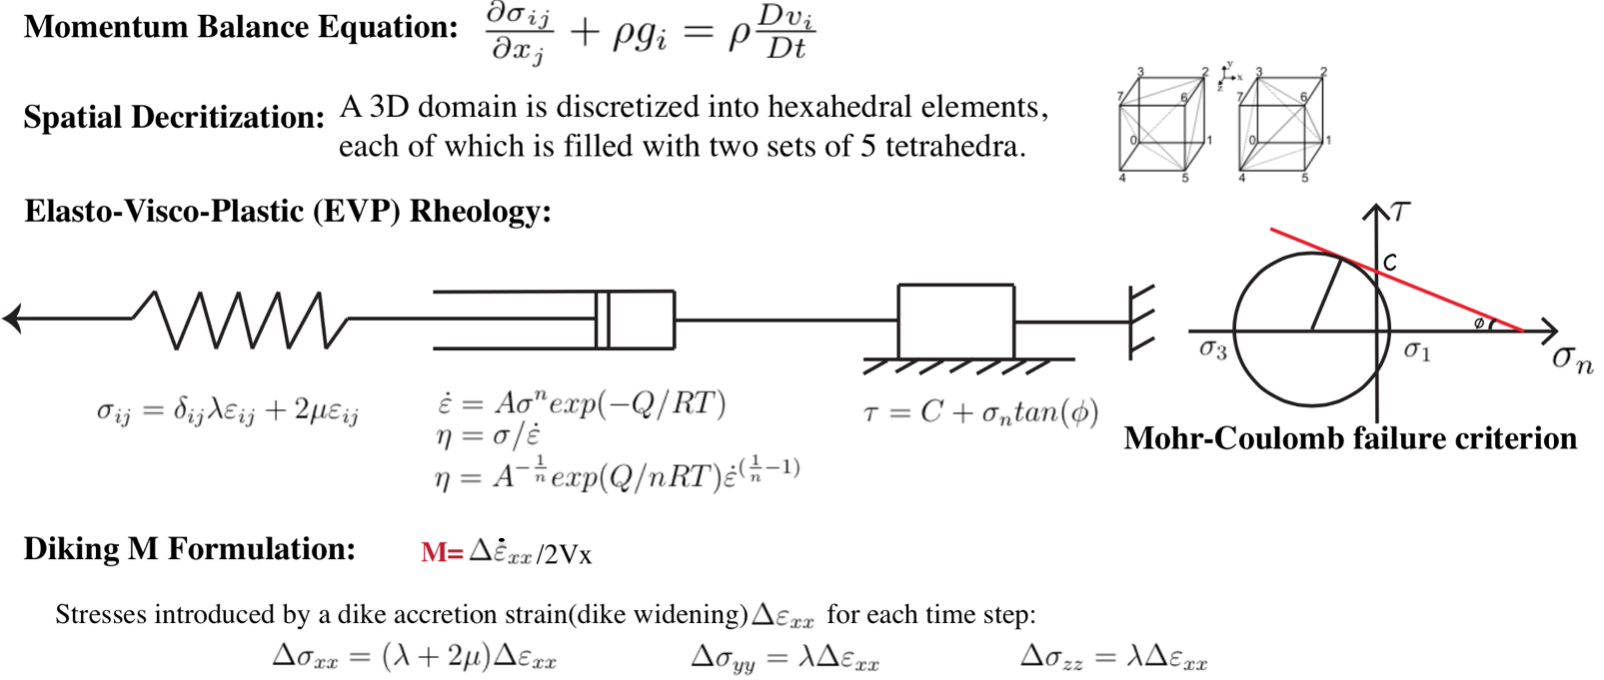
\includegraphics[scale=0.65]{fig_Methods7_2.png}
  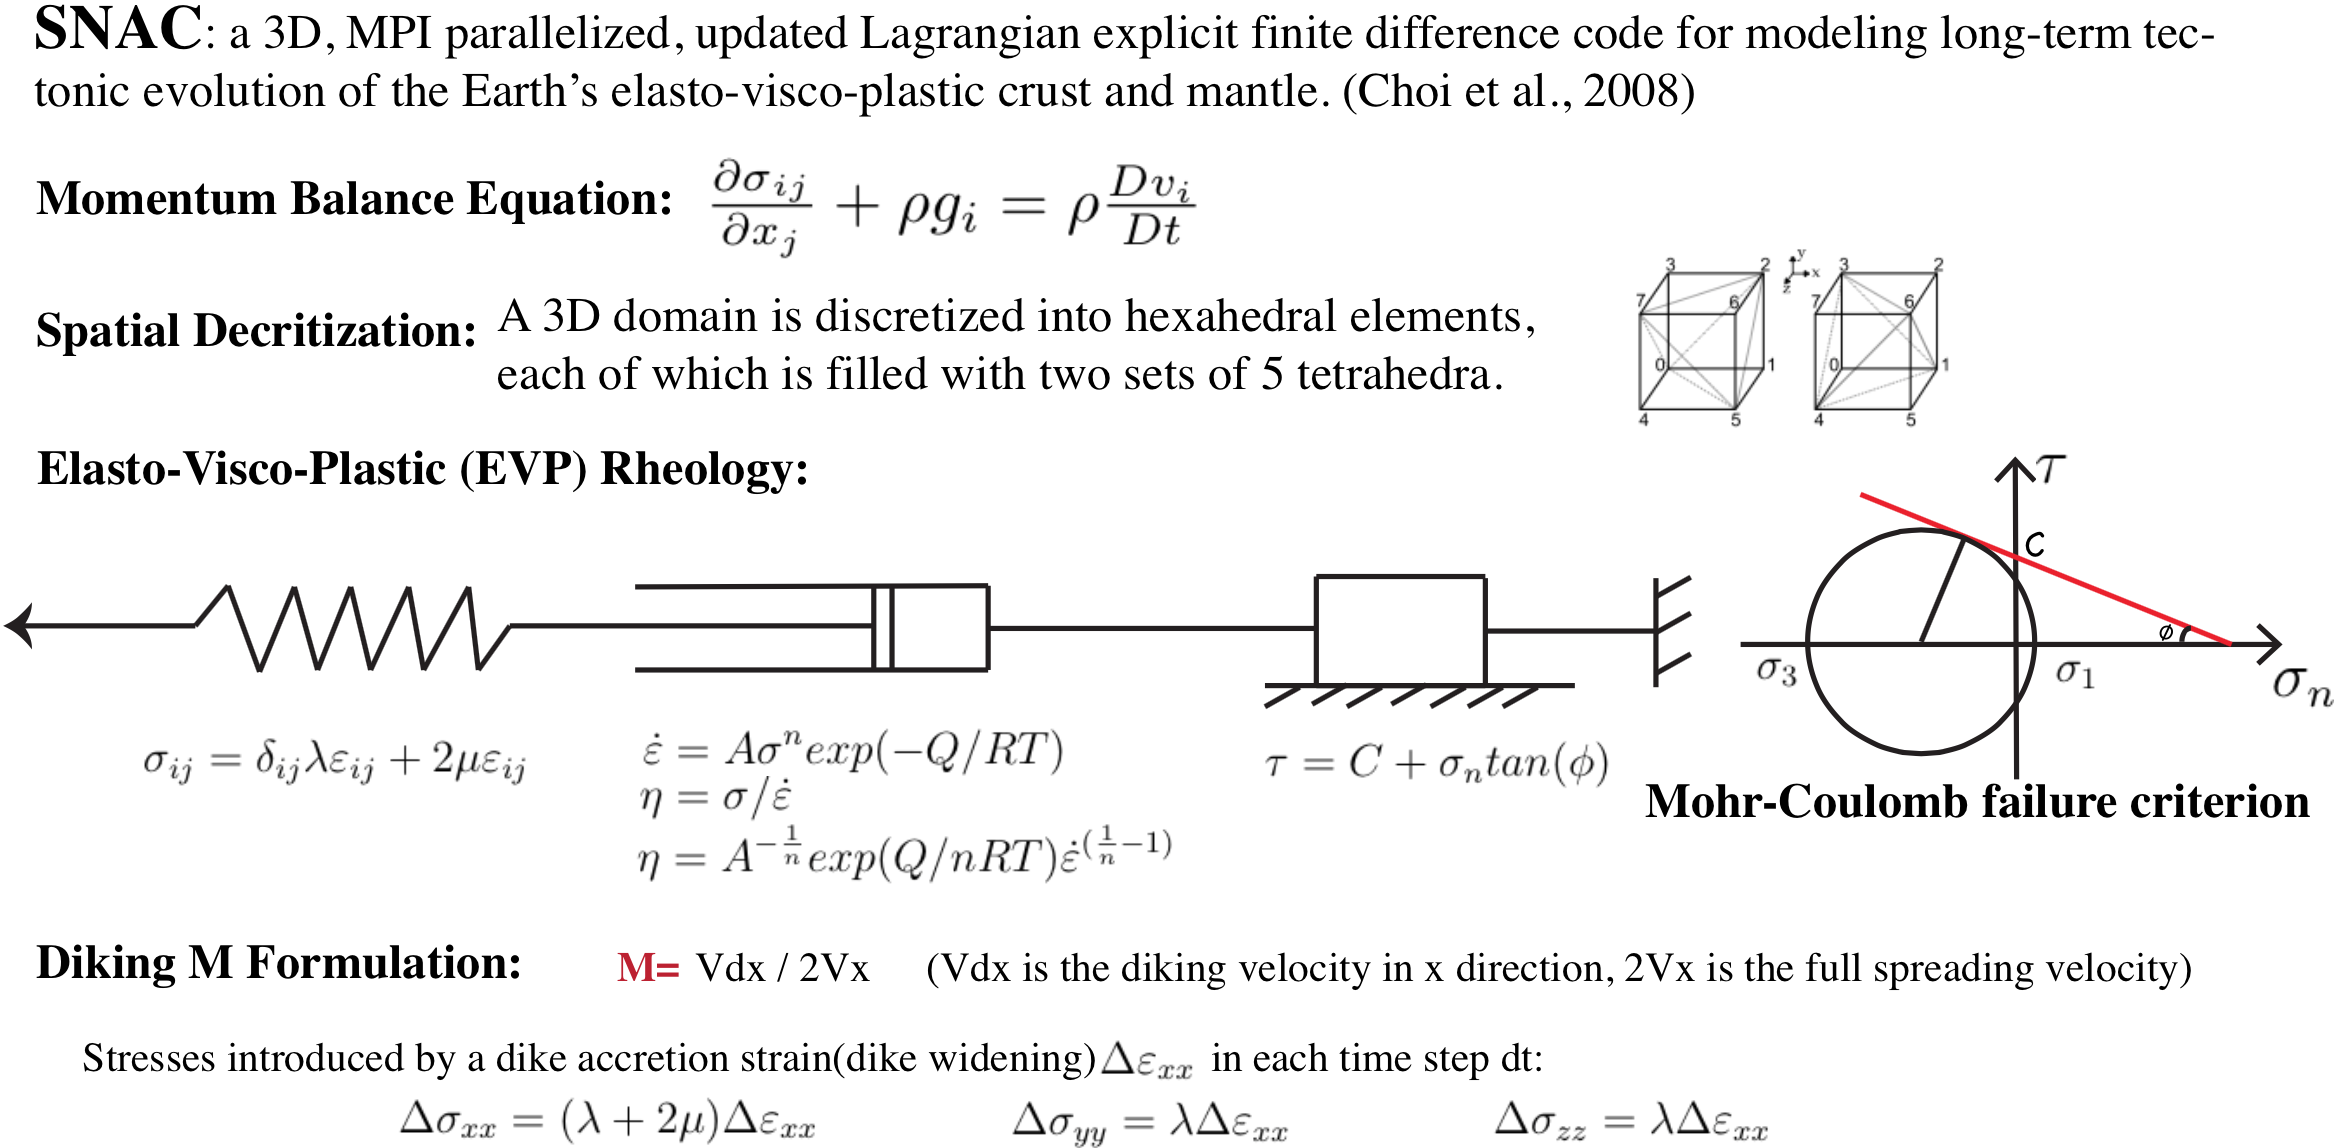
\includegraphics[width=1.0\textwidth]{fig_Methods7_3.png}
 \caption{\small{Essential components of the numerical method to be used for the proposed research}}
 \label{fig_Methods7_3}
\end{figure}

\subsection{Model Setup}
\add[XT]{Add a table for parameters in use.}
The 3D models has a geometry of ($60km \times 20km \times 20km$) in X, Y and Z axes respectively with a resolution of dx$=1km$ (dx is the length scale for each hexahedron element). For pseudo-2D models, they have a geometry of ($60km \times 20km \times 1km$) in X, Y and Z axes respectively with a resolution of dx$=0.5km$. As shown in Figure~\ref{fig_Methods8_1}, temperature linearly increases from 0 \degree C at the top surface to 240 \degree C at the depth of 6 km, reflecting enhanced cooling due to hydrothermal circulation. Below 6 km, the temperature profile follows the semi-infinite half-space cooling model of moving plates \citep[e.g.,][]{Turcotte2002}. Two sides perpendicular to the $z$ coordinate axis are free-slip. The top surface has a vertical traction from water column, of which height is locally determined as 4000-h(x,z) m, where h(x,z) is the topography at a location, (x,z). The bottom surface is supported by the Winkler foundation. Temperature is fixed at 0\degree C on the top surface and at 1300\degree C on the bottom surface. We will adopt the power-law rheology of dry diabase\citep[e.g.,][]{Kirby1987, Buck2005}. 

For detail model parameters, please refer to Table~\hyperref[Tab_ModelParameters]{\ref{Tab_ModelParameters}}.

\begin{figure}[H]
 \centering
%  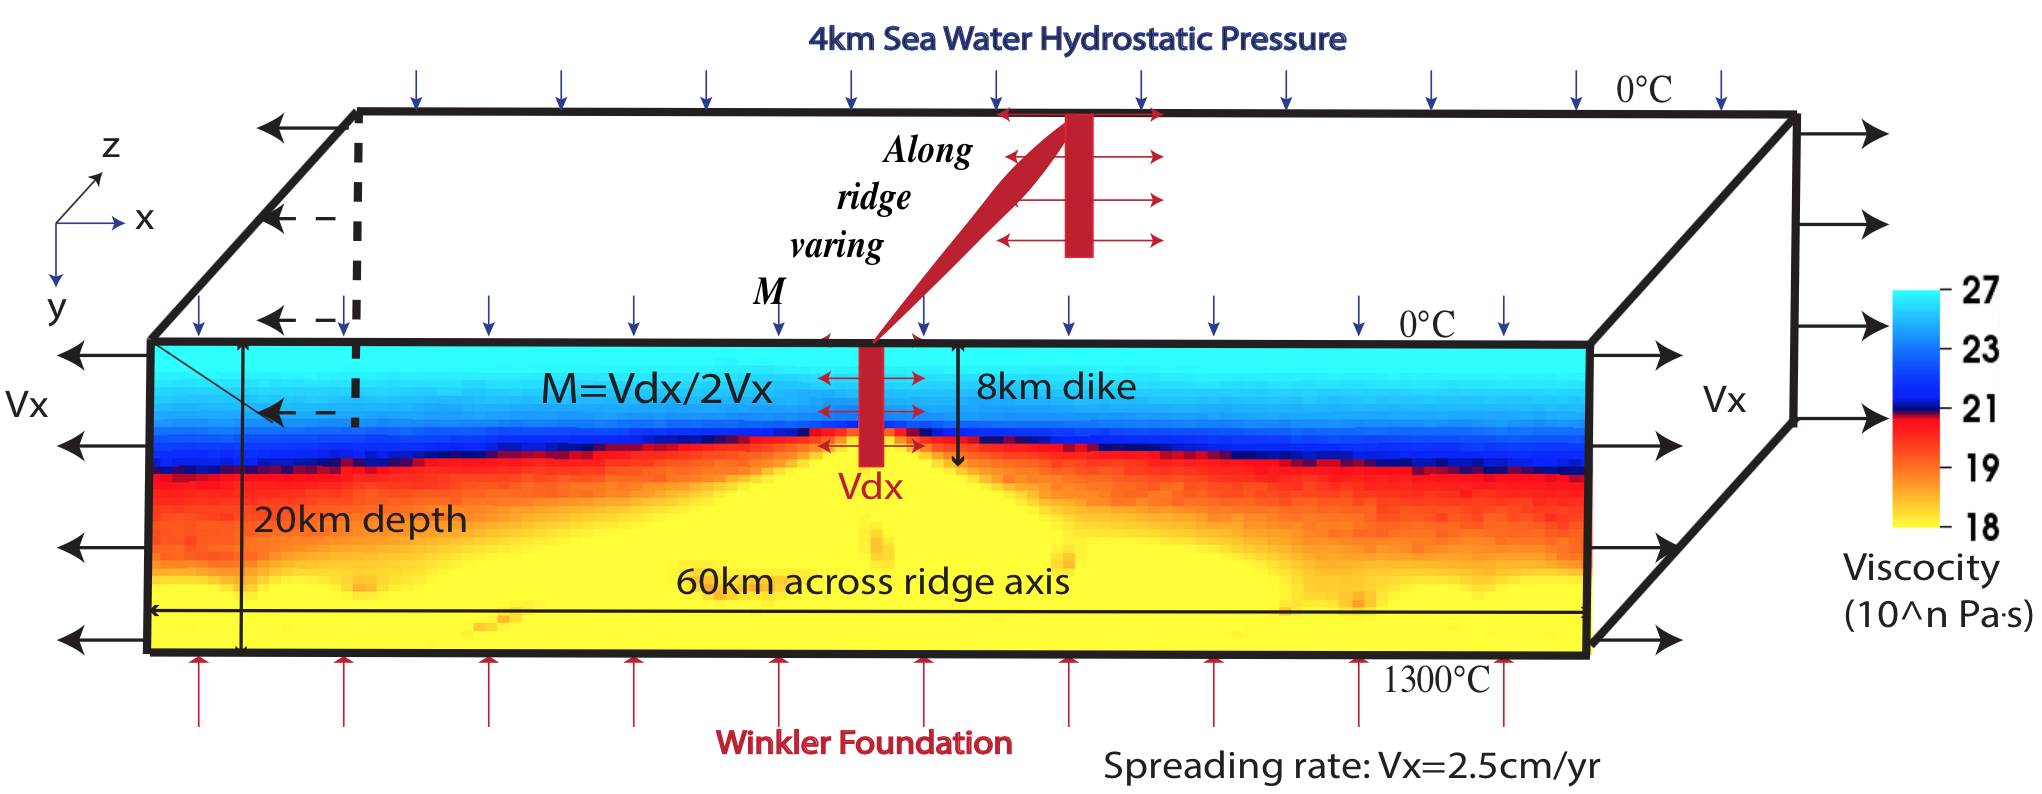
\includegraphics[scale=0.55]{fig_Methods8_1.png}
  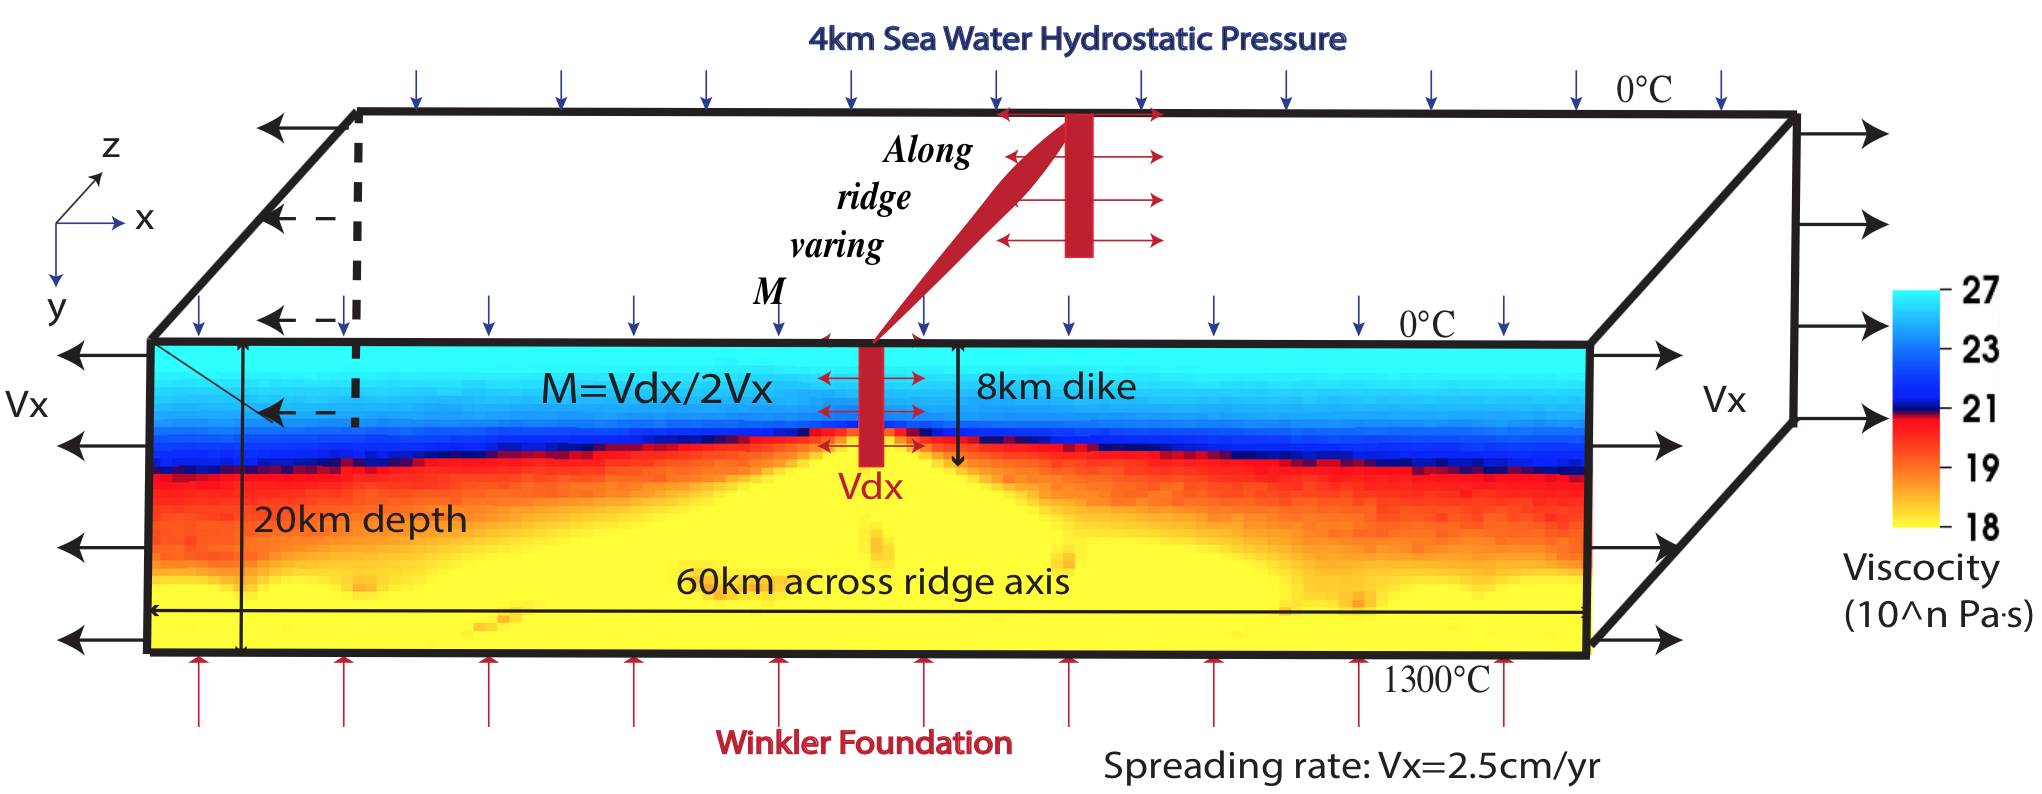
\includegraphics[width=1.0\textwidth] {fig_Methods8_1.png}
 \caption{\small Model setup}
 \label{fig_Methods8_1}
\end{figure}


\begin{table}[h]
 \centering
 \small
  \begin{tabular}[h]{l l p{6.8cm} l l}
\hline
\hline
Number & Variable & Description & Value & Units \\ 
\hline
1    &  $W_{dike}$    &   Dike width        & 2   &  $km$\\
\hline
2    &  $D_{dike}$    &   Dike depth        & 8   &  $km$\\
\hline
3    &  $H$    &   Crustal thickness at dike   & 6   &  $km$ \\
\hline
4    &  $dT/dy$    &   Crustal thermal gradient        & 40   &  $K/km$ \\
\hline
5    &  $T_{1}$    &   Temperature at lower boundary of crust    & 240   &  $\degree C$ \\
\hline
6    &  $g$    &   Gravity acceleration    & 10   &  $m/s^{2}$ \\
\hline
7    &  $demf$    &   Dimensionless force damping factor   & 0.8   &  N/A  \\
\hline
8    &  $dt$    &   Time step    & 1.5768e+07   &  $second$  \\
\hline
9    &  $topo_kappa$    &   Parameter for topography smoothing    & 0   &  N/A   \\
\hline
10   &  $shadowDepth$    &   Ghost elements for parallel computing   & 2   &  N/A   \\
\hline
11   &  $meshI$    &   Mesh number in X direction   & 60   &  N/A   \\
\hline
12   &  $meshJ$    &   Mesh number in Y direction      & 20   & N/A  \\
\hline
13   &  $meshK$    &   Mesh number in Z direction      & 20   & N/A  \\
\hline
14   &  $L_{I}$    &   Length in X direction      & 20   & $km$  \\
\hline
15   &  $L_{J}$    &   Length in Y direction      & 20   & $km$  \\
\hline
16   &  $L_{K}$    &   Length in Z direction      & 20   & $km$  \\
\hline
17   &  $\rho$    &    Density      & 3000   & $kg/m^{3}$  \\
\hline
18   &  $\lambda$    &    Lam$\acute{e}$'s constant      & 30   & $Gpa$  \\
\hline
19   &  $\mu$    &    Shear modulus      & 30   & $Gpa$  \\
\hline
20   &  $refvisc$    &    Reference viscosity      & 0.125e-17   & $Pa^{-n}/s$  \\
\hline
21   &  $activationE$    &    Activation Energy      & 276.0e+3   & $kJ/mol$  \\
\hline
22   &  $vis_{min}$    &    viscosity minimum cutoff      & 1.0e+18   & $Pa*s$  \\
\hline
23   &  $vis_{max}$    &    viscosity maximum cutoff      & 1.0e+27   & $Pa*s$  \\
\hline
24   &  $srexponent$    &    Power of power law in viscosity       & 3.05   & N/A  \\
\hline
25   &  $\varepsilon_{p_{i}}^{1}$    &    initial plastic strain for piecewise Type one weakening       & $0$   & N/A  \\
\hline
26   &  $\varepsilon_{p_{i}}^{2}$    &    initial plastic strain for piecewise Type two weakening       & $0$   & N/A  \\
\hline
27   &  $\varepsilon_{p_{e}}^{1}$    &    end plastic strain for piecewise Type one weakening       & $0.1$   & N/A  \\
\hline
28   &  $\varepsilon_{p_{e}}^{2}$    &    end plastic strain for piecewise Type two weakening       & $0.33$   & N/A  \\
\hline
29   &  $C_{i}$    &    initial Cohesion for piecewise weakening       & 44   & $Mpa$  \\
\hline
30   &  $C_{e}$    &    end Cohesion for piecewise weakening       & 4   & $Mpa$  \\
\hline
31   &  $\phi$    &    Friction angle      & 30   & $\degree$  \\
\hline
32   &  $remesh_{timestep}$    &    Remesh when timestep reach its value      & 400000   & N/A  \\
\hline
33   &  $remesh_{length}$    &    Remesh when ratio between current global minimum of the ratio of a tetrahedron’s volume to one of its surface area to its initial value      & 0.6   & N/A  \\
\hline
34   &  $top_{Temp}$    &    Surface temperature      & 0   & $\degree C$  \\
\hline
35   &  $bottom_{Temp}$    &    Bottom temperature      & 1300   & $\degree C$  \\
\hline
36   &  $V_{x}$    &    Half spreading rate      & 7.9e-10   & $m/s$  \\

\hline
\hline
\end{tabular}

\caption{Summary of 3D Model Parameters}
\label{Tab_ModelParameters}
\end{table}

\subsection{Parameters to control}
Although how to estimate the M values from observations has not been well established, we do have constraints from a large dataset of bathymetry, gravity and seismic surveys as well as geological drilling. Generally, at slow spreading ridges, magma supplies mostly at the center of the ridge segment and decreases towards the end of the segment \citep{Tolstoy1993,Chen1999}. There is also evidence for shorter wavelength of 10 to 20 km discrete focus of magma accretion along the ridge axis \citep{Lin1990}. 

Based on these constraints, we can start considering only a few end-member scenarios of variations in M along the ridge axis. The variation in M is parametrized in terms of the functional forms (e.g. discrete increment, linear, sinusuidal and square root), its wavelength (e.g. 10km, 20km and 40km) and the ranges of M (e.g. 0.2 to 0.8, 0.5 to 0.7 and 0.5 to 0.8). 

Preliminary pseudo-2D results show that the model behavior in faulting pattern is sensitive to the rate of strain weakening. Two cases of strain weakening are tested in this study. In one case (denoted as Type 1), cohesion linearly decreases from 44 MPa (denoted as $C_{i}$) to 4 MPa ($C_{e}$) for plastic strain accumulating from 0 ($\varepsilon_{p_{i}}$) to 0.1 ($\varepsilon_{p_{e}}$). It has a characteristic fault slip of 150 meters for pseudo-2D models and 300 meters for 3D models. The other case (Type 2) assumes cohesion linearly decreasing from 44 MPa to 4 MPa for plastic strain accumulating from 0 to 0.33. In this case, the characteristic fault slip for Pseudo-2D models is 500 meters and for 3D models is 1km.

The characteristic fault slip $\Delta X_{c}=3 \times dx \times \varepsilon_{p_{e}}$ (3 is because the thickness of the shear bands is usually 2 to 4 times of the dx \citep{Lavier2000}) means when $\Delta X_{c}$ amount of displacement takes place at the fault interface, the Cohesion of the material at the faulting interface will decrease to $C_{e}$. In this way, under same amount of $\Delta X_{c}$, models with different resolution should behave in the same way in terms of strain weakening and faulting patterns. 

